\documentclass[12pt]{article}
\usepackage[a4paper,margin=1.7cm]{geometry}
\usepackage{fontspec}
\usepackage{hyperref}
\usepackage{enumitem}
\usepackage{titlesec}
\usepackage{setspace}
\usepackage{xcolor}
\usepackage{parskip}
\usepackage{tikz}
\usepackage{fancyhdr}
\usepackage{tabularx}
\usepackage{array}
\usepackage{graphicx}
\usepackage{booktabs}
\usepackage{multicol}
\usetikzlibrary{arrows.meta,positioning,shapes.geometric,fit,backgrounds,calc}

\setmainfont{TeX Gyre Pagella}
\setsansfont{TeX Gyre Heros}
\setmonofont{DejaVu Sans Mono}
\emergencystretch=3em

\definecolor{ink}{HTML}{172534}
\definecolor{miku}{HTML}{39C5BB}
\definecolor{mikuDeep}{HTML}{169E95}
\definecolor{mist}{HTML}{F7FBFC}
\definecolor{line}{HTML}{D4E3E7}
\definecolor{blush}{HTML}{F6DCE9}
\definecolor{lavender}{HTML}{EDE8FA}
\definecolor{stone}{HTML}{6A7685}

\hypersetup{
  colorlinks=true,
  linkcolor=mikuDeep,
  urlcolor=mikuDeep,
  pdftitle={ARI Founder Book v1.1},
  pdfauthor={GitHub Copilot}
}

\pagestyle{fancy}
\fancyhf{}
\fancyhead[L]{\sffamily\textcolor{stone}{ARI Founder Book v1.1}}
\fancyhead[R]{\sffamily\textcolor{stone}{\thepage}}
\renewcommand{\headrulewidth}{0pt}
\setlength{\headheight}{15pt}

\setstretch{1.12}
\setlist[itemize]{leftmargin=1.45em,itemsep=0.24em,topsep=0.28em}
\setlist[enumerate]{leftmargin=1.65em,itemsep=0.24em,topsep=0.28em}

\titleformat{\section}
  {\Large\sffamily\bfseries\color{ink}}
  {}
  {0em}
  {}
  [\vspace{0.3em}\color{miku}\rule{\linewidth}{0.8pt}]

\titleformat{\subsection}
  {\large\sffamily\bfseries\color{ink}}
  {}
  {0em}
  {}

\titleformat{\subsubsection}
  {\normalsize\sffamily\bfseries\color{ink}}
  {}
  {0em}
  {}

\newcommand{\chapterquote}[1]{
  \vspace{0.4em}
  \begin{center}
  \fcolorbox{line}{mist}{\parbox{0.93\linewidth}{\sffamily\small\textcolor{stone}{#1}}}
  \end{center}
  \vspace{0.2em}
}

\newcommand{\tastebox}[2]{
  \vspace{0.45em}
  \fcolorbox{line}{mist}{\parbox{0.95\linewidth}{\sffamily\textbf{\textcolor{ink}{#1}}\\[0.2em]\normalfont\color{ink}#2}}
  \vspace{0.35em}
}

\newcommand{\signalbox}[2]{
  \vspace{0.45em}
  \fcolorbox{miku!25}{miku!8}{\parbox{0.95\linewidth}{\sffamily\textbf{\textcolor{mikuDeep}{#1}}\\[0.2em]\normalfont\color{ink}#2}}
  \vspace{0.35em}
}

\newcommand{\softbox}[2]{
  \vspace{0.45em}
  \fcolorbox{blush!70!line}{blush!30}{\parbox{0.95\linewidth}{\sffamily\textbf{\textcolor{ink}{#1}}\\[0.2em]\normalfont\color{ink}#2}}
  \vspace{0.35em}
}

\renewcommand{\contentsname}{Book Map}

\begin{document}

\begin{titlepage}
\thispagestyle{empty}
\begin{tikzpicture}[remember picture,overlay]
  \fill[mist] (current page.south west) rectangle (current page.north east);
  \fill[miku!10] ($(current page.north east)+(-6.5,-1.5)$) circle (3.3cm);
  \fill[blush!50] ($(current page.north east)+(-2.2,-4.2)$) circle (2.0cm);
  \fill[lavender!55] ($(current page.south west)+(3.0,3.8)$) circle (2.6cm);
  \fill[miku!20] ($(current page.south west)+(1.3,8.8)$) circle (1.4cm);
  \draw[line, line width=0.8pt] ($(current page.north west)+(1.2,-1.2)$) rectangle ($(current page.south east)+(-1.2,1.2)$);
\end{tikzpicture}

\vspace*{2.2cm}

{\sffamily\Large\textcolor{mikuDeep}{ARI}}\\[0.4cm]
{\sffamily\fontsize{26}{30}\selectfont\bfseries\textcolor{ink}{Founder Book v1.1}}\\[0.35cm]
{\sffamily\Large\textcolor{stone}{Purpose, Taste, Architecture, and Execution}}\\[1.0cm]

\fcolorbox{line}{white}{\parbox{0.78\linewidth}{
\sffamily\color{ink}
This book is designed for a founder-researcher who wants more than inspiration. Its job is to train judgment: what is worth building, what is not, and how to distinguish deep work from fashionable performance.
}}\\[1.2cm]

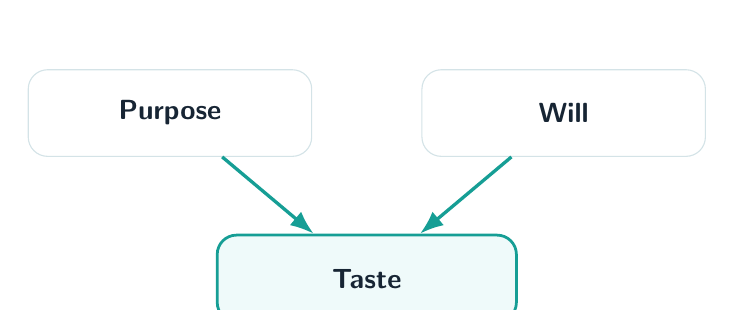
\begin{tikzpicture}[x=1cm,y=1cm]
  \node[draw=line, fill=white, rounded corners=7pt, minimum width=3.6cm, minimum height=1.1cm, text=ink, font=\sffamily\bfseries] (p) at (0,0) {Purpose};
  \node[draw=line, fill=white, rounded corners=7pt, minimum width=3.6cm, minimum height=1.1cm, text=ink, font=\sffamily\bfseries] (w) at (5.0,0) {Will};
  \node[draw=mikuDeep, fill=miku!8, rounded corners=7pt, minimum width=3.8cm, minimum height=1.1cm, line width=1.0pt, text=ink, font=\sffamily\bfseries] (t) at (2.5,-2.1) {Taste};
  \draw[-{Latex[length=3mm]}, line width=1.2pt, color=mikuDeep] (p) -- (t);
  \draw[-{Latex[length=3mm]}, line width=1.2pt, color=mikuDeep] (w) -- (t);
\end{tikzpicture}

\vfill

{\sffamily\large\textcolor{stone}{March 13, 2026}}\\[0.2cm]
{\sffamily\small\textcolor{stone}{Designed for long-horizon thinking in the AI age}}
\end{titlepage}

\tableofcontents
\newpage

\section{Why This Book Exists}

\chapterquote{Purpose decides what is worth your life. Will decides whether you can endure. Taste decides whether you are climbing the right mountain.}

This book is not here to make you sound sophisticated. It is here to make you harder to fool.

In the AI era, information is abundant, generation is cheap, and performance can look like substance. The scarce thing is not output. The scarce thing is judgment.

Taste, in this context, is not preference. It is the ability to distinguish:

\begin{itemize}
  \item signal from noise
  \item mechanism from metaphor
  \item durable leverage from passing novelty
  \item trustworthy systems from impressive demos
  \item civilizational infrastructure from product theater
\end{itemize}

\signalbox{Practical definition}{If purpose tells you what kind of future is worth serving, taste tells you which paths are real enough, deep enough, and worthy enough to justify years of your life.}

\section{The Founder's Map}

Large ambitions fail when they are compressed into a single word like AI, robotics, or biotech. The right map has layers, and each layer disciplines the one above it.

\begin{center}
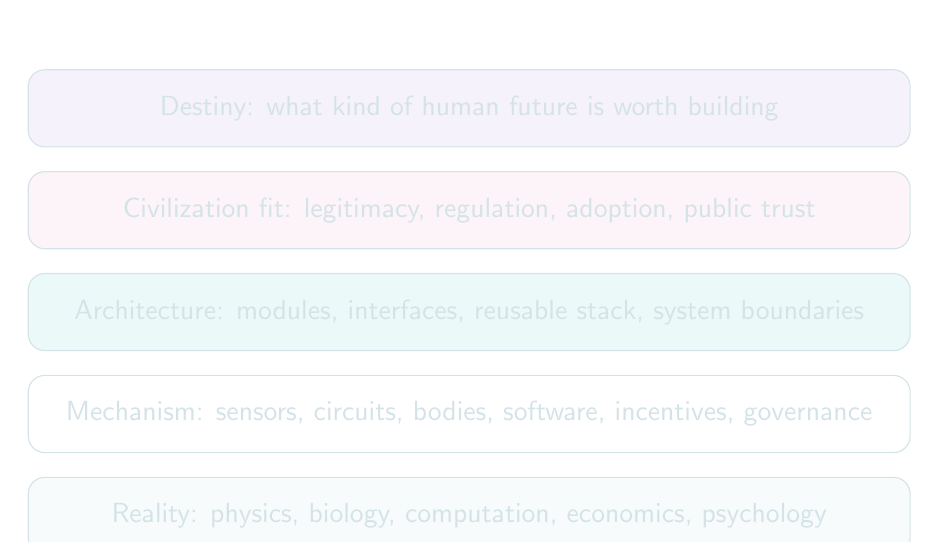
\begin{tikzpicture}[
  layer/.style={draw=line, rounded corners=6pt, fill=white, minimum width=11.2cm, minimum height=0.98cm, align=center, font=\sffamily},
  every path/.style={color=line}
]
  \node[layer, fill=lavender!55] (e) at (0,0) {Destiny: what kind of human future is worth building};
  \node[layer, fill=blush!32, below=0.3cm of e] (d) {Civilization fit: legitimacy, regulation, adoption, public trust};
  \node[layer, fill=miku!10, below=0.3cm of d] (c) {Architecture: modules, interfaces, reusable stack, system boundaries};
  \node[layer, fill=white, below=0.3cm of c] (b) {Mechanism: sensors, circuits, bodies, software, incentives, governance};
  \node[layer, fill=mist, below=0.3cm of b] (a) {Reality: physics, biology, computation, economics, psychology};
\end{tikzpicture}
\end{center}

If any one of these layers is ignored, the vision becomes fiction.

\tastebox{Founder standard}{A serious founder does not only ask whether something can be built. A serious founder asks whether it fits reality, compounds architecturally, survives institutions, and improves human life with dignity.}

\section{How Taste Is Built}

Taste is built by repeated contact with reality and repeated refusal of shallowness.

\subsection{Five habits that train taste}

\begin{enumerate}
  \item Ask what is invariant. Energy, latency, incentives, trust boundaries, and embodiment keep returning across cycles.
  \item Prefer mechanism over metaphor. Ask what the state variables are, what update rule changes them, and what fails first.
  \item Learn to see interfaces. Most systems do not break inside modules. They break where modules meet.
  \item Study failure without contempt. Scientific falsehood, weak engineering, wrong economics, or missing social contract each teach different lessons.
  \item Build small things that expose deep truths. Small systems are where reality stops letting you bluff.
\end{enumerate}

\softbox{Refusal is part of taste}{Taste grows as much by what you reject as by what you pursue. If you never consciously refuse a seductive but shallow direction, your standards are probably too soft.}

\section{Knowledge System to Rebuild}

If rebuilding from a high-school starting point, the cleanest order is:

\begin{enumerate}
  \item mathematics as the language of structure and change
  \item physics and dynamical systems
  \item computer science as controlled complexity
  \item neuroscience and computation
  \item embodiment and robotics
  \item biology and augmentation
  \item institutions, privacy, and inequality
\end{enumerate}

\subsection{Good taste while learning}

\begin{itemize}
  \item connect formulas to mechanisms
  \item keep asking what a concept lets you model
  \item care about interfaces, not just modules
  \item notice recurring constraints across fields
  \item prefer clarity over ceremonial sophistication
\end{itemize}

\subsection{Bad taste while learning}

\begin{itemize}
  \item memorizing terms you cannot operationalize
  \item jumping to fashionable topics before learning constraints
  \item treating biology like software and society like a late-stage add-on
  \item calling a diagram an architecture before defining trust boundaries
\end{itemize}

\section{Twelve Weeks That Build Momentum}

The first 12 weeks are not for mastery. They are for installing rhythm, rigor, and self-respect.

\signalbox{Weekly law}{Every week should contain study, implementation, writing, and reflection. If one disappears, your development becomes distorted.}

\subsection{Weeks 1 to 4: Language of modeling}

\begin{tabularx}{\linewidth}{>{\sffamily\bfseries}p{2.05cm} X}
Week 1 & Functions, variables, units, and basic modeling. Build tiny scripts for growth, decay, and threshold systems. Write why a model is a compressed causal story. \\
Week 2 & Derivatives, integration, and state updates. Implement Euler integration and observe how step size changes results. \\
Week 3 & Vectors, matrices, and uncertainty. Build a small recurrent update and add noisy sensory observations. \\
Week 4 & LIF from scratch. Sweep threshold and time constant, then write what the model preserves and what it throws away. \\
\end{tabularx}

\subsection{Weeks 5 to 8: Spikes, circuits, and bodies}

\begin{tabularx}{\linewidth}{>{\sffamily\bfseries}p{2.05cm} X}
Week 5 & Synaptic filtering, coding, excitation, inhibition. Compare fast and slow synapses. \\
Week 6 & Recurrent motifs, competition, and stability. Learn to distinguish genuine dynamics from parameter abuse. \\
Week 7 & Embodiment and feedback. Run the prototype and alter body parameters to see how behavior changes. \\
Week 8 & Connectomes and structure-constrained models. Redraw the network as sensory, interneuron, descending, and motor groups. \\
\end{tabularx}

\subsection{Weeks 9 to 12: Learning, interfaces, and founder synthesis}

\begin{tabularx}{\linewidth}{>{\sffamily\bfseries}p{2.05cm} X}
Week 9 & Plasticity and local learning. Implement one toy plasticity rule and track weights over time. \\
Week 10 & Interfaces and hidden arbitrariness. Audit which parts are principled and which are hand-tuned. \\
Week 11 & Privacy, trust, and human stakes. Design a toy privacy-first memory system and map abuse paths. \\
Week 12 & Architecture synthesis. Write one-page memos for Alive, Realize, Innocence, and the shared reusable stack. \\
\end{tabularx}

\section{A Taste Filter for Research and Product Directions}

Before committing deeply, run the direction through six tests.

\begin{center}
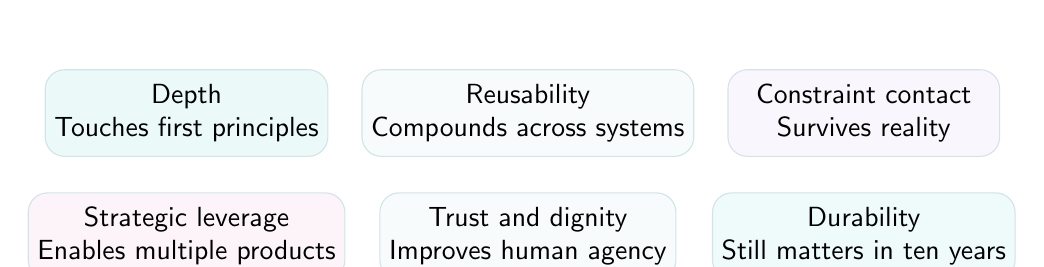
\begin{tikzpicture}[
  box/.style={draw=line, rounded corners=7pt, fill=white, minimum width=3.45cm, minimum height=1.1cm, align=center, font=\sffamily},
  node distance=0.45cm and 0.42cm
]
  \node[box, fill=miku!10] (d1) {Depth\\Touches first principles};
  \node[box, fill=mist, right=of d1] (d2) {Reusability\\Compounds across systems};
  \node[box, fill=lavender!35, right=of d2] (d3) {Constraint contact\\Survives reality};
  \node[box, fill=blush!30, below=of d1] (d4) {Strategic leverage\\Enables multiple products};
  \node[box, fill=mist, below=of d2] (d5) {Trust and dignity\\Improves human agency};
  \node[box, fill=miku!8, below=of d3] (d6) {Durability\\Still matters in ten years};
\end{tikzpicture}
\end{center}

If a direction fails several of these tests, treat it with suspicion even if everyone around you sounds excited.

\section{ARI as Three Interlocking Systems}

ARI becomes stronger when each project constrains the others and the underlying stack compounds beneath them.

\begin{center}
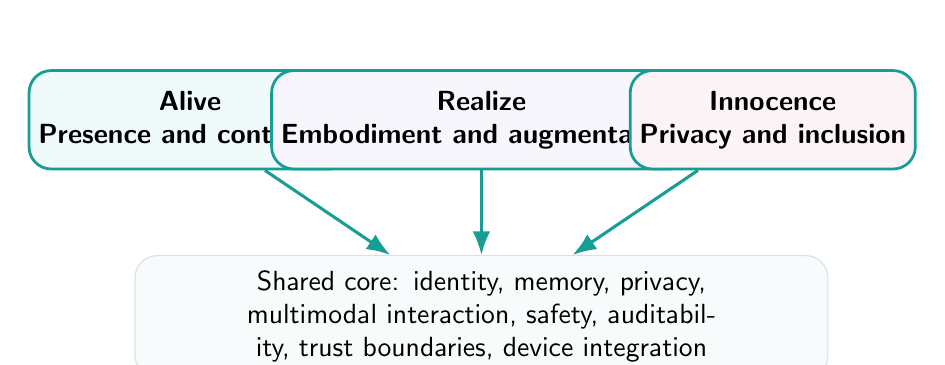
\begin{tikzpicture}[
  proj/.style={draw=mikuDeep, rounded corners=8pt, minimum width=3.55cm, minimum height=1.25cm, align=center, line width=1pt, font=\sffamily\bfseries, fill=white},
  core/.style={draw=line, rounded corners=8pt, minimum width=8.8cm, minimum height=1.55cm, align=center, fill=mist, text width=8.0cm, font=\sffamily}
]
  \node[proj, fill=miku!8] (alive) at (-3.7,1.6) {Alive\\Presence and continuity};
  \node[proj, fill=lavender!40] (realize) at (0,1.6) {Realize\\Embodiment and augmentation};
  \node[proj, fill=blush!35] (innocence) at (3.7,1.6) {Innocence\\Privacy and inclusion};
  \node[core] (core) at (0,-0.9) {Shared core: identity, memory, privacy, multimodal interaction, safety, auditability, trust boundaries, device integration};
  \draw[-{Latex[length=3mm]}, line width=1.1pt, color=mikuDeep] (alive) -- (core);
  \draw[-{Latex[length=3mm]}, line width=1.1pt, color=mikuDeep] (realize) -- (core);
  \draw[-{Latex[length=3mm]}, line width=1.1pt, color=mikuDeep] (innocence) -- (core);
\end{tikzpicture}
\end{center}

\subsection{Alive}

\textbf{Core human problem}

Loneliness is not just absence of messages. It is absence of continuity, witnessed identity, and trusted presence.

\textbf{Irreducible technical object}

Not a chatbot, but a persistent relational agent with memory, boundaries, and continuity.

\textbf{Minimum architecture}

\begin{enumerate}
  \item identity layer
  \item memory layer
  \item multimodal interaction layer
  \item user sovereignty layer
  \item trust and safety layer
\end{enumerate}

\tastebox{Alive taste standard}{Prefer continuity over novelty, agency over dependency, and truthful relationship architecture over engagement theater.}

\subsection{Realize}

\textbf{Core human problem}

Biological limits appear as disability, decline, suffering, and hard capability ceilings.

\textbf{Irreducible technical object}

Not an enhancement slogan, but a closed-loop augmentation or restoration system grounded in measurable biology.

\textbf{Minimum architecture}

\begin{enumerate}
  \item sensing layer
  \item interpretation layer
  \item intervention layer
  \item validation layer
  \item human factors layer
\end{enumerate}

\tastebox{Realize taste standard}{Prefer mechanism over spectacle, translational seriousness over futurist language, and safety envelopes over aggressive promises.}

\subsection{Innocence}

\textbf{Core human problem}

Systemic inequality persists when infrastructure is opaque, extractive, and easy to weaponize against the weak.

\textbf{Irreducible technical object}

Not a fairness dashboard, but a privacy-first coordination and service infrastructure that preserves agency under power asymmetry.

\textbf{Minimum architecture}

\begin{enumerate}
  \item identity and consent layer
  \item data boundary layer
  \item orchestration layer across institutions
  \item accessible interface layer
  \item governance resilience layer
\end{enumerate}

\tastebox{Innocence taste standard}{Prefer privacy by architecture over policy theater, accessibility over designer self-congratulation, and hard trust boundaries over benevolent assumptions.}

\section{Shared Stack Blueprint}

The real compounding advantage of ARI depends on reusable layers, not three unrelated codebases.

\begin{center}
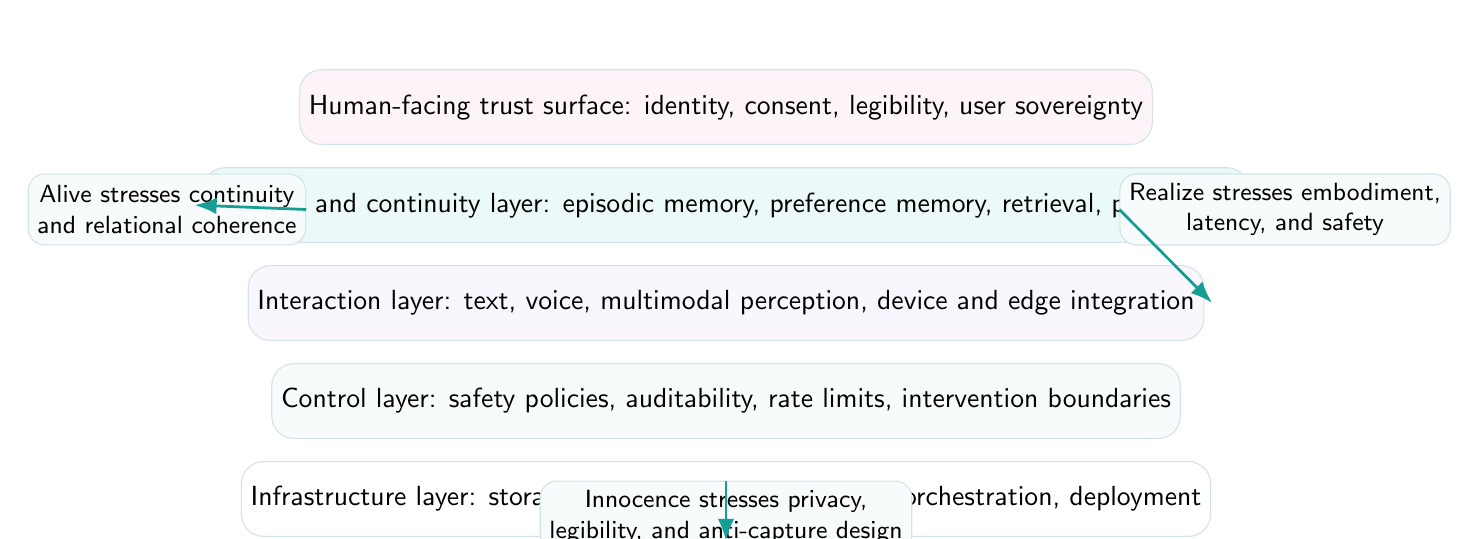
\begin{tikzpicture}[
  layer/.style={draw=line, rounded corners=8pt, minimum width=10.2cm, minimum height=0.95cm, align=center, font=\sffamily, fill=white},
  note/.style={draw=line, rounded corners=6pt, minimum width=3.2cm, minimum height=0.9cm, align=center, font=\sffamily\small, fill=mist}
]
  \node[layer, fill=blush!30] (l1) at (0,0) {Human-facing trust surface: identity, consent, legibility, user sovereignty};
  \node[layer, fill=miku!10, below=0.28cm of l1] (l2) {Memory and continuity layer: episodic memory, preference memory, retrieval, provenance};
  \node[layer, fill=lavender!35, below=0.28cm of l2] (l3) {Interaction layer: text, voice, multimodal perception, device and edge integration};
  \node[layer, fill=mist, below=0.28cm of l3] (l4) {Control layer: safety policies, auditability, rate limits, intervention boundaries};
  \node[layer, fill=white, below=0.28cm of l4] (l5) {Infrastructure layer: storage, encryption, access control, orchestration, deployment};

  \node[note] (n1) at (-7.1,-1.3) {Alive stresses continuity\\and relational coherence};
  \node[note] (n2) at (7.1,-1.3) {Realize stresses embodiment,\\latency, and safety};
  \node[note] (n3) at (0,-5.2) {Innocence stresses privacy,\\legibility, and anti-capture design};

  \draw[-{Latex[length=2.8mm]}, color=mikuDeep, line width=1pt] (n1.east) -- ($(l2.west)+(-0.1,0.0)$);
  \draw[-{Latex[length=2.8mm]}, color=mikuDeep, line width=1pt] (n2.west) -- ($(l3.east)+(0.1,0.0)$);
  \draw[-{Latex[length=2.8mm]}, color=mikuDeep, line width=1pt] (n3.north) -- ($(l5.south)+(0.0,-0.05)$);
\end{tikzpicture}
\end{center}

\begin{center}
\begin{tabularx}{\linewidth}{>{\sffamily\bfseries\raggedright\arraybackslash}p{2.25cm} >{\raggedright\arraybackslash}X >{\raggedright\arraybackslash}p{2.8cm}}
\toprule
Layer & Why it exists & Primary risk if weak \\
\midrule
Identity and sovereignty & Gives the person continuity, control, and legible boundaries across all products & dependence on opaque platform identity \\
Privacy and consent & Prevents convenience from quietly eroding agency & surveillance, capture, and silent data asymmetry \\
Personal memory & Makes continuity and personalization durable across time & inconsistency, manipulation, or memory lock-in \\
Multimodal interaction & Connects text, voice, perception, and devices into one coherent surface & fragmented experience and brittle trust \\
Safety and auditability & Makes sensitive systems inspectable and governable & latent harm with no accountable trace \\
Device and edge integration & Grounds intelligence in bodies, sensors, and local context where needed & shallow software-only claims detached from reality \\
\bottomrule
\end{tabularx}
\end{center}

\signalbox{Blueprint question}{Whenever a new feature appears, ask: is this a reusable layer, or only a local flourish? Founders with weak taste duplicate stacks. Founders with strong taste build cores that compound.}

\section{Founder Operating Principles}

These principles are meant to be used operationally, not admired abstractly.

\begin{center}
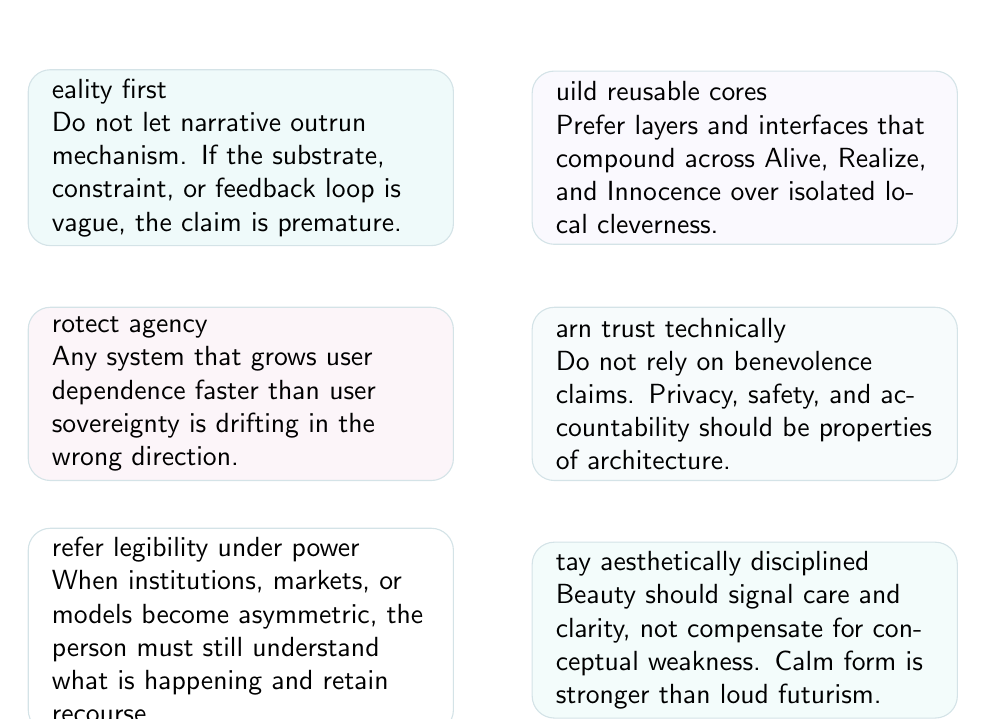
\begin{tikzpicture}[
  card/.style={draw=line, rounded corners=8pt, minimum width=5.4cm, minimum height=2.2cm, text width=4.8cm, align=left, font=\sffamily, fill=white},
  title/.style={font=\sffamily\bfseries\color{ink}}
]
  \node[card, fill=miku!8] (c1) at (-3.2,0) {{\title Reality first}\\Do not let narrative outrun mechanism. If the substrate, constraint, or feedback loop is vague, the claim is premature.};
  \node[card, fill=lavender!28] (c2) at (3.2,0) {{\title Build reusable cores}\\Prefer layers and interfaces that compound across Alive, Realize, and Innocence over isolated local cleverness.};
  \node[card, fill=blush!28] (c3) at (-3.2,-3.0) {{\title Protect agency}\\Any system that grows user dependence faster than user sovereignty is drifting in the wrong direction.};
  \node[card, fill=mist] (c4) at (3.2,-3.0) {{\title Earn trust technically}\\Do not rely on benevolence claims. Privacy, safety, and accountability should be properties of architecture.};
  \node[card, fill=white] (c5) at (-3.2,-6.0) {{\title Prefer legibility under power}\\When institutions, markets, or models become asymmetric, the person must still understand what is happening and retain recourse.};
  \node[card, fill=miku!6] (c6) at (3.2,-6.0) {{\title Stay aesthetically disciplined}\\Beauty should signal care and clarity, not compensate for conceptual weakness. Calm form is stronger than loud futurism.};
\end{tikzpicture}
\end{center}

\softbox{Operating use}{When making a serious product or research decision, it is worth asking which of these six principles the decision strengthens and which one it quietly violates.}

\section{Aesthetic and Moral Doctrine}

Beauty matters because it reveals care, restraint, and clarity. But beauty without truth becomes theater.

For a project like ARI, aesthetics should signal:

\begin{itemize}
  \item precision rather than aggression
  \item intimacy without manipulation
  \item warmth without sentimentality
  \item modernity without trend dependence
  \item trust without bureaucratic heaviness
\end{itemize}

This is why a restrained design language matters. It keeps the work from collapsing into startup bombast or sterile futurism.

\softbox{Design doctrine}{The right visual language for a civilizational project should feel lucid, humane, technically competent, and emotionally controlled. It should not need to shout.}

\section{Strategic Refusals}

Taste also grows by refusal.

\begin{multicols}{2}
\begin{itemize}
  \item refuse systems optimized mainly for hype visibility
  \item refuse moats that are mostly narrative rather than architecture
  \item refuse any design that scales dependency faster than agency
  \item refuse safety stories that depend on everyone behaving well
  \item refuse abstractions that hide the real bottleneck
  \item refuse emotional products that cannot state their ethical boundary clearly
  \item refuse biological ambition that outruns validation discipline
  \item refuse inclusion rhetoric without technical enforcement
\end{itemize}
\end{multicols}

\section{How to Use This Book}

Read it in loops rather than as a one-time artifact.

\begin{enumerate}
  \item Read once quickly for orientation.
  \item Read again with a pen and mark what feels true, vague, unfinished, or naive.
  \item Convert one section into a working memo.
  \item Convert one memo into an experiment, architecture draft, or refusal list.
  \item Re-read after reality pushes back and see what still survives.
\end{enumerate}

\signalbox{Use it correctly}{Do not use this book as identity decoration. Use it as a compression of standards that should become stricter as your contact with reality improves.}

\section{Final Standard}

Choose work that is simultaneously:

\begin{itemize}
  \item real
  \item deep
  \item reusable
  \item worthy
\end{itemize}

Alive should make companionship more real, not more addictive.

Realize should make augmentation more grounded, not more theatrical.

Innocence should make infrastructure more trustworthy, not more rhetorical.

If a technical choice strengthens those standards, it is probably aligned. If it weakens them, it is probably a distraction even if it is fashionable.

\end{document}